% ============================================================
%  Chương 3: Phương pháp thực hiện
% ============================================================

Chương này trình bày cách hiện thực hệ thống từ các nền tảng lý thuyết đã nêu ở Chương~\ref{c:cosolythuyet}. Nội dung chương đi theo luồng từ kiến trúc tổng thể, lớp thiết bị, lớp truyền thông, lớp xử lý, đến lớp ứng dụng và triển khai bằng Docker Compose. Trọng tâm của chương sẽ làm rõ cách mô hình LSTM được xây dựng như một bộ dự báo theo chuỗi thời gian và cách thuật toán PPO được dùng làm bộ điều khiển hành động.

\section{Tổng quan kiến trúc hệ thống}

Hệ thống được thiết kế theo kiến trúc 4 lớp phân tầng rõ ràng, giúp tách biệt vai trò giữa các thành phần và hỗ trợ mở rộng độc lập:

\begin{enumerate}
  \item Lớp thiết bị: ESP32 hoặc bộ mô phỏng phần mềm thu thập và gửi dữ liệu cảm biến.
  \item Lớp truyền thông: Mosquitto MQTT broker và dịch vụ cầu nối MQTT-Kafka.
  \item Lớp xử lý: Apache Spark Structured Streaming tích hợp bộ dự báo LSTM và bộ điều khiển PPO.
  \item Lớp ứng dụng: API Node.js, bảng điều khiển web, Grafana và Telegram bot.
\end{enumerate}

Sơ đồ tổng thể kiến trúc 4 tầng kèm luồng dữ liệu giữa các thành phần được thể hiện trong Hình~\ref{fig:architecture}.

\begin{center}
  \makebox[\textwidth][c]{%
    \hspace*{-1.7cm}%
    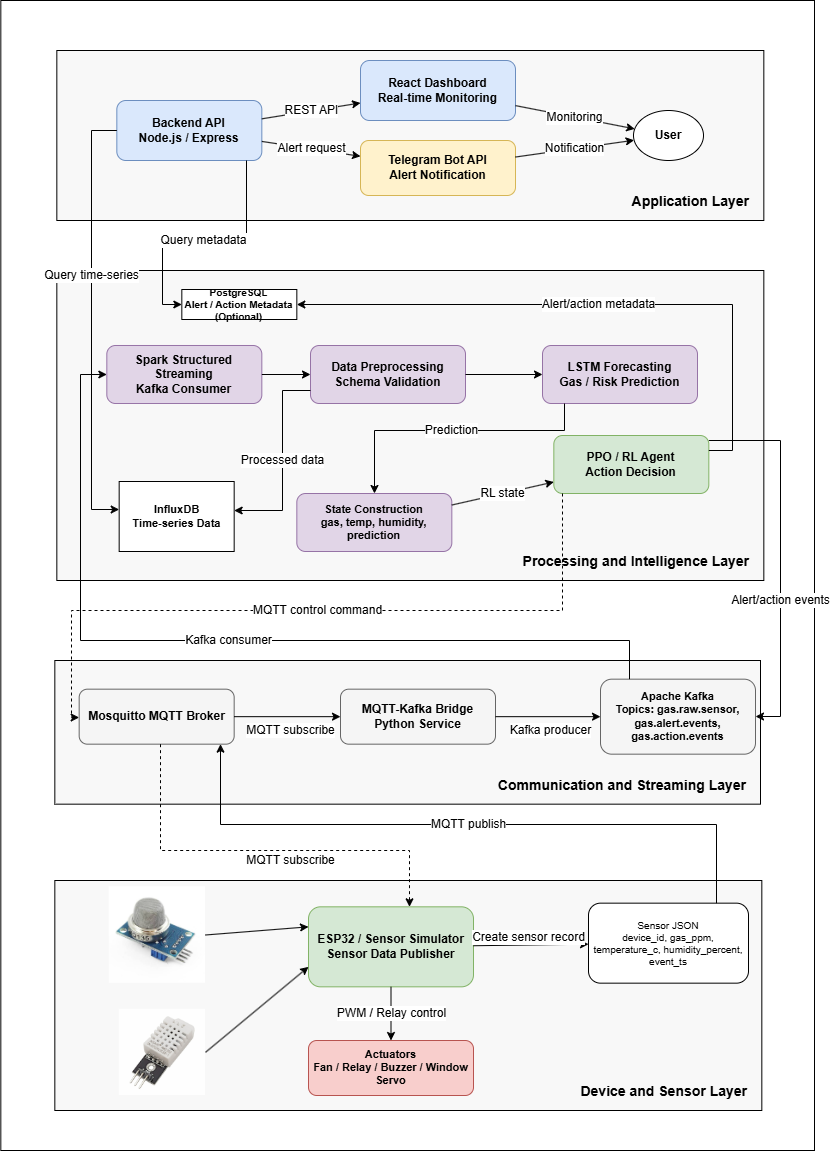
\includegraphics[
      width=1.95\textwidth,
      height=0.95\textheight,
      keepaspectratio
    ]{img/system design.png}%
  }

  \captionof{figure}{Kiến trúc hệ thống 4 tầng.}
  \label{fig:architecture}
\end{center}

\section{Lớp thiết bị}

\subsection{Chương trình ESP32}

Firmware ESP32 được viết bằng ngôn ngữ C++ sử dụng Arduino framework với thư viện PubSubClient cho MQTT. ESP32 đọc dữ liệu từ:
\begin{itemize}
  \item Cảm biến MQ (qua cổng ADC): nồng độ khí gas (ppm)
  \item Cảm biến DHT22: nhiệt độ (°C) và độ ẩm (\%)
\end{itemize}

Mỗi giây (1 Hz), chương trình ESP32 đóng gói dữ liệu thành JSON và gửi lên topic \texttt{sensors/gas}:

\Needspace{12\baselineskip}
\begin{lstlisting}[language=Python, caption={Cấu trúc payload JSON từ thiết bị}]
{
  "device_id": "esp32-lab-01",
  "gas_ppm": 125.43,
  "temperature_c": 28.12,
  "humidity_percent": 61.5,
  "event_ts": 1703123456789
}
\end{lstlisting}

\subsection{Bộ mô phỏng cảm biến}

Do điều kiện thực nghiệm, bộ mô phỏng phần mềm được xây dựng để thay thế phần cứng trong quá trình huấn luyện mô hình và đánh giá so sánh. Bộ mô phỏng triển khai một máy trạng thái vật lý với 4 trạng thái:

\begin{itemize}
  \item NORMAL: Nồng độ nền 50–150 ppm, dao động Gaussian nhỏ. Hàm cập nhật:
  \[gas_t = gas_{t-1} + 0.1(60 - gas_{t-1}) \cdot dt + \mathcal{N}(0, 3) \cdot dt\]

  \item LEAK\_SLOW: Rò rỉ chậm, tốc độ tăng tuyến tính $\sim$5 ppm/s:
  \[gas_t = gas_{t-1} + 5 \cdot dt + \mathcal{N}(0, 2) \cdot dt\]

  \item LEAK\_FAST: Rò rỉ nhanh (vỡ ống), tăng theo hàm mũ:
  \[gas_t = gas_{t-1} \cdot e^{0.04 \cdot dt} + 8 \cdot dt + \mathcal{N}(0, 3) \cdot dt\]

  \item VENTILATING: Sau khi có hành động can thiệp, khí giảm theo hàm mũ:
  \[gas_t = \max(60, gas_{t-1} \cdot e^{-0.03 \cdot dt} - 0.5 \cdot dt)\]
\end{itemize}

Xác suất chuyển trạng thái ngẫu nhiên được tham số hóa qua biến môi trường \texttt{SIM\_LEAK\_PROB\_PER\_MIN} (mặc định 5\% mỗi phút). Trong pha NORMAL, 70\% trường hợp chuyển sang LEAK\_SLOW và 30\% chuyển sang LEAK\_FAST.

Bộ mô phỏng cũng gửi kèm hai trường nhãn thực tế:
\begin{itemize}
  \item \texttt{\_leak\_state}: Trạng thái thực tế (chỉ dùng cho đánh giá).
  \item \texttt{\_seconds\_to\_critical}: Số giây đến khi nồng độ đạt 1000 ppm (ước tính).
\end{itemize}

\section{Lớp truyền thông}

\subsection{Mosquitto MQTT Broker}

Mosquitto là MQTT broker mã nguồn mở nhẹ của Eclipse Foundation. Trong hệ thống, Mosquitto được cấu hình:
\begin{itemize}
  \item Cổng 1883 cho kết nối không mã hóa trong mạng Docker nội bộ.
  \item Bật lưu trạng thái để không mất bản tin khi broker khởi động lại.
  \item Không giới hạn số kết nối trong môi trường phát triển.
\end{itemize}

\subsection{MQTT-Kafka Bridge}

Dịch vụ cầu nối (\texttt{mqtt\_kafka\_bridge.py}) đóng vai trò chuyển bản tin giữa hai giao thức:

\Needspace{12\baselineskip}
\begin{lstlisting}[language=Python, caption={Logic bridge đơn giản hóa}]
def on_message(client, userdata, msg):
    payload = json.loads(msg.payload)
    # Validate and add metadata
    payload['ingested_at'] = int(time.time() * 1000)
    # Chuyen tiep sang Kafka
    producer.produce(
        topic='gas.raw.sensor',
        key=payload['device_id'],
        value=json.dumps(payload),
        callback=delivery_report
    )
    producer.poll(0)
\end{lstlisting}

Dịch vụ cầu nối đăng ký nhận dữ liệu từ MQTT topic \texttt{sensors/gas} và chuyển tiếp lên Kafka topic \texttt{gas.raw.sensor}. Trường \texttt{device\_id} được dùng làm khóa để giữ đúng thứ tự bản tin của từng thiết bị trong Kafka partition.

\section{Lớp xử lý}

\subsection{Luồng xử lý Spark Structured Streaming}

File \texttt{stream\_processor.py} là điểm vào của lớp xử lý. Luồng Spark được thiết kế theo các bước:

Bước 1 – Đọc từ Kafka:
\Needspace{12\baselineskip}
\begin{lstlisting}[language=Python, caption={Đọc luồng dữ liệu từ Kafka}]
raw_stream = (
    spark.readStream
    .format("kafka")
    .option("kafka.bootstrap.servers", KAFKA_BROKERS)
    .option("subscribe", "gas.raw.sensor")
    .option("startingOffsets", "latest")
    .load()
)
\end{lstlisting}

Bước 2 – Phân tích JSON và trích xuất đặc trưng:

Mỗi bản ghi được phân tích từ JSON. Để đưa dữ liệu vào LSTM (cần chuỗi 60 giây), luồng xử lý duy trì một cửa sổ trượt cho từng \texttt{device\_id} trong bộ nhớ. Python UDF nhận chuỗi hiện tại và gọi bộ dự báo:

\Needspace{10\baselineskip}
\begin{lstlisting}[language=Python, caption={Gọi bộ dự báo LSTM trong Spark}]
@udf(returnType=FloatType())
def predict_risk(gas, temp, hum):
    return forecaster.predict(device_id, gas, temp, hum)
\end{lstlisting}

Bước 3 – Gọi bộ điều khiển PPO:

Sau khi có xác suất rủi ro từ LSTM, Spark gọi tác nhân PPO để chọn hành động:

\begin{lstlisting}[language=Python, caption={Gọi tác nhân PPO}]
action, action_name = rl_agent.choose(
    device_id, gas, temp, hum, predicted_risk
)
\end{lstlisting}

Bước 4 – Ghi kết quả:
\begin{itemize}
  \item Ghi vào InfluxDB measurement \texttt{gas\_readings} mọi bản ghi kèm xác suất rủi ro và hành động.
  \item Nếu action $\neq$ NO\_OP, gửi sự kiện lên Kafka topic \texttt{gas.alert.events}.
\end{itemize}

\subsection{Bộ dự báo LSTM}

\subsubsection*{Kiến trúc mô hình}

Mô hình LSTM dự báo được xây dựng bằng Keras/TensorFlow với kiến trúc nhỏ gọn phù hợp với suy luận thời gian thực:

\begin{lstlisting}[
language=Python,
caption={Định nghĩa kiến trúc LSTM},
breaklines=true,
breakatwhitespace=true,
postbreak=\mbox{\textcolor{red}{$\hookrightarrow$}\space}
]
inp = tf.keras.layers.Input(shape=(60, 3))
x = tf.keras.layers.LSTM(32, return_sequences=False)(inp)
x = tf.keras.layers.Dropout(0.2)(x)
x = tf.keras.layers.Dense(16, activation="relu")(x)
out = tf.keras.layers.Dense(1, activation="sigmoid")(x)
model = tf.keras.Model(inp, out)
model.compile(
    optimizer=Adam(1e-3),
    loss="binary_crossentropy",
    metrics=["accuracy", Precision(), Recall()]
)
\end{lstlisting}

Hàm mất mát \texttt{binary\_crossentropy} được dùng vì nhãn huấn luyện là nhãn \emph{dự báo sự kiện}: cửa sổ hiện tại có dẫn đến trạng thái vượt ngưỡng trong 5 phút tới hay không. Đây không phải là bài toán gán nhãn trạng thái tức thời. Nếu mục tiêu được đổi thành dự báo trực tiếp giá trị \texttt{gas\_ppm} tại các thời điểm tương lai, khi đó cần dùng các hàm mất mát và tiêu chí hồi quy như MAE hoặc RMSE.

Tổng số tham số: $\sim$5,000 -- đủ nhỏ để suy luận trong vài millisecond. Sơ đồ khối các lớp được mô tả ở Hình~\ref{fig:lstm_arch} (Chương~\ref{c:cosolythuyet}).

\subsubsection*{Quy trình huấn luyện}

Sinh dữ liệu: Chạy bộ mô phỏng trong $N$ giờ (mặc định 4 giờ) với seed cố định để tạo trace xác định. Trace có dạng mảng $(T, 4)$: $(gas, temp, hum, state\_int)$.

Xây dựng dataset: Với mỗi vị trí $i$ trong trace:
\begin{itemize}
  \item $X[i]$ = chuỗi 60 giây chuẩn hóa kết thúc tại $t$: $feats[i:i+60] / [2000, 60, 100]$
  \item $y[i] = 1$ nếu $\max(gas[i+61:i+361]) > 1000$ else $0$
\end{itemize}

Phân chia train/test: Phân chia theo thứ tự thời gian (80/20), không xáo trộn để tránh data leakage.

Xử lý mất cân bằng: Áp dụng class weight với hệ số:
\[w_{pos} = \frac{1 - p_{pos}}{p_{pos}}, \quad w_{neg} = 1.0\]

trong đó $p_{pos}$ là tỷ lệ mẫu positive trong tập huấn luyện.

\subsubsection*{Hai phiên bản mô hình LSTM được huấn luyện}
\label{sssec:lstm_two_models}

Một điểm cần làm rõ ở mức triển khai là trong đề tài, \emph{cùng một kiến trúc} LSTM (Hình~\ref{fig:lstm_arch}) được huấn luyện thành hai mô hình riêng biệt. Cả hai mô hình đều được đóng gói trong thư mục \texttt{processing/ml/lstm/}, nhưng phục vụ hai mục tiêu đánh giá khác nhau:

\begin{enumerate}
  \item Mô hình mô phỏng (\texttt{gas\_forecaster.keras}): được huấn luyện trên trace 8 giờ sinh từ bộ mô phỏng với seed cố định. Đây là bộ dự báo \emph{mặc định} được nạp trong luồng Spark, do nhãn rò rỉ được xác định rõ và phân phối dữ liệu phù hợp với môi trường mô phỏng dùng để đánh giá so sánh các bộ điều khiển.

  \item Mô hình dữ liệu thực (\texttt{gas\_forecaster\_kaggle.keras}): được huấn luyện trên tập dữ liệu cảm biến IoT thực từ Kaggle. Mô hình này không dùng làm bộ dự báo mặc định trong luồng mô phỏng, mà được sử dụng để kiểm chứng sơ bộ khả năng tổng quát hóa của kiến trúc LSTM trên dữ liệu cảm biến thực.
\end{enumerate}

Bảng~\ref{tab:lstm_two_models} đối chiếu cấu hình huấn luyện của hai mô hình. Điểm mấu chốt là kiến trúc mạng, hàm mất mát và cách xây dựng nhãn theo hướng \emph{dự báo sự kiện} được giữ nhất quán giữa hai mô hình; sự khác biệt chủ yếu nằm ở nguồn dữ liệu, ngưỡng sinh nhãn và một số siêu tham số huấn luyện. Nhờ vậy, kết quả trên tập dữ liệu thực Kaggle có thể được xem là bằng chứng bổ trợ cho thấy kiến trúc LSTM đề xuất có khả năng học xu hướng biến thiên của tín hiệu khí trong nhiều nguồn dữ liệu khác nhau, thay vì chỉ phù hợp với riêng dữ liệu sinh ra từ bộ mô phỏng.

\begingroup
\small
\renewcommand{\arraystretch}{1.25}
\setlength{\tabcolsep}{4pt}

\begin{longtable}{
  >{\raggedright\arraybackslash}p{2.8cm}
  >{\raggedright\arraybackslash}p{5.0cm}
  >{\raggedright\arraybackslash}p{5.0cm}
}
\caption{Đối chiếu hai mô hình LSTM cùng kiến trúc}
\label{tab:lstm_two_models} \\
\toprule
\textbf{Hạng mục} 
& \textbf{Mô hình mô phỏng} 
& \textbf{Mô hình dữ liệu thực (Kaggle)} \\
\midrule
\endfirsthead

% Không lặp lại header nếu bảng bị cắt sang trang mới
\endhead

\bottomrule
\endlastfoot

File trọng số   
& \texttt{gas\_forecaster.keras} 
& \texttt{gas\_forecaster\_kaggle.keras} \\

Nguồn dữ liệu   
& Trace mô phỏng 8\,h, tần số 1\,Hz, seed 42 
& Kaggle Env. Sensor, khoảng 405K mẫu, 3 thiết bị \\

Đặc trưng đầu vào 
& Cửa sổ 60 $\times$ (gas, T, H) 
& Cửa sổ 60 $\times$ (lpg, temp, humidity) \\

Ngưỡng dán nhãn 
& Gas tương lai $> 1000$\,ppm 
& LPG tương lai $> \mathrm{LPG}_{p95}$ \\

Kiến trúc mạng  
& \multicolumn{2}{
    >{\raggedright\arraybackslash}p{10.0cm}
  }{
    \emph{Giống nhau}: Input(60,3) $\rightarrow$ LSTM(32) $\rightarrow$ Dropout(0{,}2) $\rightarrow$ Dense(16) $\rightarrow$ Dense(1)
  } \\

Epochs / batch  
& 20 / 128 
& 25 / 256 \\

Vai trò         
& Bộ dự báo vận hành mặc định 
& Kiểm chứng sơ bộ trên dữ liệu thực \\

\end{longtable}
\endgroup

\subsubsection*{Cơ chế fallback}

Khi mô hình Keras chưa được huấn luyện (file \texttt{.keras} chưa tồn tại), bộ dự báo tự động dùng cơ chế dự phòng bằng ngoại suy xu hướng. Cơ chế này ước tính độ dốc tuyến tính trên 30 mẫu gần nhất bằng \texttt{numpy.polyfit}, sau đó thực hiện ngoại suy tới chân trời $H=300$\,giây. Nếu độ dốc vượt 0{,}5 ppm/s, cơ chế dự phòng bổ sung thêm nhánh ngoại suy mũ bằng cách ước lượng hệ số tăng trưởng trung bình trên 15 mẫu cuối. Giá trị dự báo cuối cùng là \texttt{max(linear, exp)} và được ánh xạ sang xác suất qua hàm logistic với biên $200$\,ppm xung quanh ngưỡng nguy hiểm. Cơ chế này đảm bảo hệ thống vẫn cho ra xác suất dự báo hợp lý ngay cả khi mô hình Keras chưa sẵn sàng, đồng thời chống lại các trường hợp tăng phi tuyến (LEAK\_FAST) mà phép ngoại suy tuyến tính sẽ đánh giá thấp.

\subsection{Bộ điều khiển PPO}

\subsubsection*{Môi trường: \texttt{GasLeakEnv}}

Bài toán điều khiển được mô hình hoá thành một quá trình quyết định Markov (MDP) gồm bốn thành phần: môi trường, không gian trạng thái, không gian hành động và hàm phần thưởng. Bốn thành phần này được trình bày lần lượt trong các mục dưới đây.

\texttt{GasLeakEnv} kế thừa từ \texttt{gymnasium.Env} và bao bọc bộ mô phỏng vật lý đã mô tả ở mục lớp thiết bị, biến nó thành một môi trường tương tác chuẩn cho thuật toán PPO: ở mỗi bước, môi trường nhận một hành động, cập nhật động lực vật lý của phòng (nồng độ khí, trạng thái rò rỉ), rồi trả về trạng thái kế tiếp và phần thưởng tương ứng.

\Needspace{0.62\textheight}
\begin{lstlisting}[
language=Python,
caption={Cấu trúc GasLeakEnv (đã được đơn giản hoá)},
basicstyle=\ttfamily\scriptsize,
lineskip=-1pt
]
class GasLeakEnv(gymnasium.Env):
    observation_space = Box(low=0.0, high=1.0, shape=(8,), dtype=np.float32)
    action_space = Discrete(4)  # NO_OP, ALERT, FAN_ON, CLOSE_VALVE

    def step(self, action):
        leaking = self.world.state in (LEAK_SLOW, LEAK_FAST)

        self._apply_action(action, leaking)
        STEP_FN[self.world.state](self.world, dt=1.0)
        self._apply_ventilation()
        _maybe_transition(self.world, dt=1.0)

        reward = self._compute_reward(action, leaking)
        done = self.t >= self.T
        return self._observe(), reward, False, done, {}
\end{lstlisting}

\subsubsection*{Không gian trạng thái}

Không gian trạng thái là một vector quan sát 8 chiều, mỗi thành phần được chuẩn hoá về $[0,1]$ để mạng policy học ổn định (chi tiết ở Bảng~\ref{tab:rl_state}). Ngoài bốn đại lượng cảm biến/dự báo (nồng độ khí, nhiệt độ, độ ẩm và độ dốc \textit{slope} ước tính trên 30 mẫu cuối) cùng đặc trưng ghép tầng $p_{5\min}$ lấy từ LSTM, trạng thái còn chứa hai cờ nội bộ của bộ điều khiển (\texttt{fan\_on}, \texttt{valve\_closed}) và thời gian kể từ hành động cuối $\Delta t_{\mathrm{act}}$. Hai cờ nội bộ cho phép policy biết các can thiệp đã được kích hoạt để tránh lặp lại không cần thiết.

\begingroup
\small
\renewcommand{\arraystretch}{1.25}
\setlength{\tabcolsep}{4pt}

\begin{longtable}{
  >{\centering\arraybackslash}p{0.8cm}
  >{\raggedright\arraybackslash}p{3.2cm}
  >{\raggedright\arraybackslash}p{8.2cm}
}
\caption{Không gian trạng thái: vector quan sát 8 chiều của \texttt{GasLeakEnv}}
\label{tab:rl_state} \\
\toprule
\textbf{\#} 
& \textbf{Thành phần} 
& \textbf{Ý nghĩa đã chuẩn hoá về $[0,1]$} \\
\midrule
\endfirsthead

% Không lặp lại header nếu bảng bị cắt sang trang mới
\endhead

% Không thêm dòng "Còn tiếp ở trang sau"
\endfoot

\bottomrule
\endlastfoot

1 
& \texttt{gas\_norm}      
& Nồng độ khí chia cho 2000. \\

2 
& \texttt{temp\_norm}     
& Nhiệt độ chia cho 60. \\

3 
& \texttt{hum\_norm}      
& Độ ẩm chia cho 100. \\

4 
& \texttt{slope\_norm}    
& Độ dốc của 30 mẫu gần nhất, được ánh xạ từ khoảng $[-10,10]$ sang $[0,1]$. \\

5 
& $p_{5\mathrm{min}}$             
& Xác suất nguy hiểm trong 5 phút tiếp theo, là đầu ra của mô hình LSTM. \\

6 
& \texttt{fan\_on}        
& Cờ trạng thái cho biết quạt đang bật hay tắt, nhận giá trị $\{0,1\}$. \\

7 
& \texttt{valve\_closed}  
& Cờ trạng thái cho biết van gas đang đóng hay mở, nhận giá trị $\{0,1\}$. \\

8 
& $\Delta t_{\mathrm{act}}$ 
& Thời gian tính từ hành động điều khiển cuối cùng, chia cho 300. \\

\end{longtable}
\endgroup

\subsubsection*{Không gian hành động}

Không gian hành động là tập rời rạc gồm 4 hành động (\texttt{Discrete(4)}); mỗi bước thời gian tác nhân chọn đúng một hành động (Bảng~\ref{tab:rl_action}). Bốn hành động có \emph{chi phí} và \emph{tác động vật lý} rất khác nhau: ALERT rẻ và không làm thay đổi quỹ đạo khí; FAN làm khí giảm chậm ($\sim$1,5\%/giây); còn CLOSE\_VALVE chặn hẳn nguồn rò rỉ nhưng đồng thời cắt nguồn cung khí của hộ gia đình nếu kích hoạt sai lúc. Chính sự bất đối xứng về chi phí này là lý do bài toán được mô hình hóa theo học tăng cường và giải bằng PPO thay vì chỉ dùng một ngưỡng cứng.

\begingroup
\small
\renewcommand{\arraystretch}{1.25}
\setlength{\tabcolsep}{4pt}

\begin{longtable}{
  >{\centering\arraybackslash}p{1.0cm}
  >{\raggedright\arraybackslash}p{3.2cm}
  >{\raggedright\arraybackslash}p{8.0cm}
}
\caption{Không gian hành động: 4 hành động rời rạc của \texttt{GasLeakEnv}}
\label{tab:rl_action} \\
\toprule
\textbf{Mã} 
& \textbf{Hành động} 
& \textbf{Tác động vật lý / chi phí} \\
\midrule
\endfirsthead

% Không lặp lại header nếu bảng bị cắt sang trang mới
\endhead

% Không thêm dòng "Còn tiếp ở trang sau"
\endfoot

\bottomrule
\endlastfoot

0 
& \texttt{NO\_OP}       
& Không làm gì, chỉ chịu chi phí theo từng bước thời gian. \\

1 
& \texttt{ALERT\_USER}  
& Gửi cảnh báo đến người dùng; chi phí thấp và không tác động trực tiếp đến môi trường vật lý. \\

2 
& \texttt{FAN\_ON}      
& Bật quạt thông gió, làm giảm nồng độ khí khoảng $1{,}5\%$/giây. \\

3 
& \texttt{CLOSE\_VALVE} 
& Đóng van gas để chặn nguồn rò rỉ. \\

\end{longtable}
\endgroup

\subsubsection*{Hàm phần thưởng}

Hàm reward được thiết kế theo nguyên tắc \textit{asymmetric cost} kết hợp \textit{outcome-based}: hậu quả của việc bỏ sót rò rỉ (gas vượt ngưỡng nguy hiểm) phải nặng hơn rất nhiều so với cảnh báo sai, và phần thưởng tích cực được trao \emph{theo kết quả} (giữ được khí dưới ngưỡng) thay vì theo hành động:

\begin{align*}
R_t = 
& -0.05 \\
& -50 \cdot \mathbf{1}[gas_t \geq 1000] \\
& +0.3 \cdot \mathbf{1}[leaking \land gas_t < 1000] \\
& + C(action_t, state_t) \\
& + H(state_t).
\end{align*}

\begingroup
\small
\renewcommand{\arraystretch}{1.25}
\setlength{\tabcolsep}{4pt}

\begin{longtable}{
  >{\raggedright\arraybackslash}p{10.2cm}
  >{\centering\arraybackslash}p{2.2cm}
}
\caption{Bộ hệ số reward tham chiếu từ code \texttt{processing/ml/rl/gas\_env.py}}
\label{tab:reward_shape} \\
\toprule
\textbf{Tình huống} 
& \textbf{Reward} \\
\midrule
\endfirsthead

% Không lặp lại header nếu bảng bị cắt sang trang mới
\endhead

% Không thêm dòng "Còn tiếp ở trang sau"
\endfoot

\bottomrule
\endlastfoot

Mỗi bước có $gas \geq 1000$\,ppm, tức hệ thống bỏ sót trạng thái nguy hiểm
& $-50$ \\

Mỗi bước đang rò rỉ nhưng vẫn giữ được $gas < 1000$\,ppm
& $+0{,}3$ \\

Hành động \texttt{ALERT\_USER} khi trạng thái môi trường là \texttt{NORMAL}, tức cảnh báo sai
& $-3$ \\

Hành động \texttt{FAN\_ON} lần đầu khi trạng thái môi trường là \texttt{NORMAL}
& $-15$ \\

Hành động \texttt{CLOSE\_VALVE} lần đầu khi trạng thái môi trường là \texttt{NORMAL}
& $-25$ \\

Giữ van gas ở trạng thái đóng trong môi trường \texttt{NORMAL}, tính theo mỗi bước thời gian
& $-0{,}5$ \\

Giữ quạt thông gió chạy trong môi trường \texttt{NORMAL}, tính theo mỗi bước thời gian
& $-0{,}1$ \\

Chi phí mặc định cho mỗi bước thời gian
& $-0{,}05$ \\

\end{longtable}
\endgroup

Thiết kế hàm thưởng này khắc phục hai vấn đề của phiên bản đầu. \emph{Thứ nhất}, phần thưởng cố định $+10$ cho mỗi lần bấm FAN/VALVE trong lúc rò rỉ bị loại bỏ vì nó cho phép tác nhân tăng điểm thưởng bằng cách lặp lại hành động mà không thực sự kiềm chế được khí, một dạng khai thác sai hàm thưởng. Thay vào đó, phần thưởng $+0{,}3$ chỉ được trao khi khí \emph{thực sự} được giữ dưới ngưỡng trong lúc rò rỉ; vì quạt không thể kiềm chế rò rỉ nhanh (tăng mũ $\sim$4\%/s, trong khi quạt chỉ giảm 1{,}5\%/s), cơ chế này buộc tác nhân học \emph{đóng van} cho LEAK\_FAST. \emph{Thứ hai}, chi phí duy trì ($-0{,}5$ giữ van, $-0{,}1$ giữ quạt trong NORMAL) cùng cơ chế tự khôi phục giúp hạn chế việc chính sách duy trì van hoặc quạt quá lâu khi môi trường đã an toàn: đóng van sai trong NORMAL ngắt nguồn cung khí gas của hộ gia đình, một thiệt hại trải nghiệm thực tế. Hệ số $-50$ cho bước vượt ngưỡng được giữ lớn để ưu tiên tuyệt đối yếu tố an toàn.

\subsubsection*{Huấn luyện PPO}

\Needspace{0.45\textheight}
\begin{lstlisting}[
language=Python,
caption={Cấu hình PPO training},
basicstyle=\ttfamily\scriptsize,
lineskip=-1pt
]
env = make_vec_env(lambda: GasLeakEnv(episode_seconds=1800),
                   n_envs=4, seed=42)
env = VecNormalize(env, norm_obs=False, norm_reward=True, clip_reward=10.0)

model = PPO("MlpPolicy", env,
            n_steps=512, batch_size=128,
            gamma=0.99, gae_lambda=0.95,
            learning_rate=3e-4, ent_coef=0.01)
model.learn(total_timesteps=400_000)
model.save("processing/ml/rl/ppo_gas_agent.zip")
\end{lstlisting}

Bảng~\ref{tab:ppo_hyperparams} tổng hợp các siêu tham số chính của quá trình huấn luyện PPO. Các giá trị này được chọn theo cấu hình ổn định của Stable-Baselines3 cho môi trường hành động rời rạc, đồng thời giữ chi phí huấn luyện phù hợp với phạm vi thực nghiệm.

\begingroup
\small
\renewcommand{\arraystretch}{1.25}
\setlength{\tabcolsep}{4pt}

\begin{longtable}{
  >{\raggedright\arraybackslash}p{3.4cm}
  >{\centering\arraybackslash}p{2.8cm}
  >{\raggedright\arraybackslash}p{6.8cm}
}
\caption{Các siêu tham số chính khi huấn luyện PPO}
\label{tab:ppo_hyperparams} \\
\toprule
\textbf{Siêu tham số} 
& \textbf{Giá trị} 
& \textbf{Ý nghĩa} \\
\midrule
\endfirsthead

% Không lặp lại header nếu bảng bị cắt sang trang mới
\endhead

% Không thêm dòng "Còn tiếp ở trang sau"
\endfoot

\bottomrule
\endlastfoot

Tổng số bước huấn luyện 
& 400{,}000 
& Số bước thời gian tác nhân tương tác với môi trường mô phỏng. \\

Số môi trường song song 
& 4 
& Tăng đa dạng trạng thái quan sát trong quá trình lấy mẫu. \\

Độ dài episode 
& 1{,}800\,s 
& Mỗi episode tương ứng 30 phút mô phỏng. \\

\texttt{n\_steps} 
& 512 
& Số bước thu thập trước mỗi lần cập nhật policy. \\

\texttt{batch\_size} 
& 128 
& Kích thước minibatch khi tối ưu PPO. \\

\texttt{gamma} 
& 0{,}99 
& Hệ số chiết khấu reward tương lai. \\

\texttt{gae\_lambda} 
& 0{,}95 
& Tham số Generalized Advantage Estimation. \\

\texttt{learning\_rate} 
& $3\times10^{-4}$ 
& Tốc độ học của optimizer. \\

\texttt{ent\_coef} 
& 0{,}01 
& Khuyến khích khám phá trong quá trình huấn luyện. \\

\end{longtable}
\endgroup

4 môi trường song song giúp tăng độ đa dạng của dữ liệu huấn luyện và giảm thời gian huấn luyện. Mỗi episode kéo dài 1800 giây (30 phút) mô phỏng. Bộ bọc \texttt{VecNormalize} chuẩn hoá reward giúp đường cong huấn luyện hội tụ rõ ràng và dễ diễn giải (xem Chương~\ref{c:thucnghiemdanhgia}), khắc phục hiện tượng reward kẹt ở vùng âm của phiên bản đầu.

Sơ đồ khối toàn bộ mạng PPO (kiến trúc actor-critic dùng \texttt{MlpPolicy} mặc định của Stable-Baselines3) được thể hiện trong Hình~\ref{fig:ppo_arch}. Phần dùng chung gồm hai lớp Dense 64 đơn vị, kích hoạt $\tanh$; trên đó tách thành hai đầu độc lập: đầu chính sách trả về phân phối xác suất trên 4 hành động qua softmax, đầu giá trị trả về giá trị $V_\phi(s)$ vô hướng. Toàn bộ mạng có khoảng 5{,}000 tham số, nhẹ tương đương bộ dự báo LSTM.

\Needspace{0.55\textheight}
\begin{center}
  \makebox[\textwidth][c]{%
    
\includegraphics[width=1.18\linewidth]{ppo_arch.png}%
  }
  \captionof{figure}{Sơ đồ khối kiến trúc PPO actor-critic sử dụng Stable-Baselines3 \texttt{MlpPolicy}.}
  \label{fig:ppo_arch}
\end{center}

\subsubsection*{Cơ chế fallback}

Tương tự LSTM, tác nhân PPO có một cơ chế dự phòng theo luật, được kích hoạt khi file PPO chưa tồn tại hoặc tải lỗi. Cơ chế dự phòng bám sát triết lý của hàm thưởng (ưu tiên an toàn, thận trọng với hành động đắt), gồm năm luật được đánh giá theo thứ tự dừng-đầu-tiên:
\begin{enumerate}
  \item Nếu $gas > 800$\,ppm và van chưa đóng $\Rightarrow$ CLOSE\_VALVE.
  \item Nếu $p_{5\min} > 0{,}7$ và van chưa đóng $\Rightarrow$ CLOSE\_VALVE.
  \item Nếu $p_{5\min} > 0{,}4$ hoặc slope $> 1$\,ppm/s, và quạt chưa bật $\Rightarrow$ FAN\_ON.
  \item Nếu $p_{5\min} > 0{,}3$ $\Rightarrow$ ALERT\_USER.
  \item Ngược lại $\Rightarrow$ NO\_OP.
\end{enumerate}
Quy tắc này tham chiếu cả nồng độ tức thời \emph{và} tín hiệu dự báo từ LSTM, đảm bảo hệ thống vẫn có khả năng phản ứng đa cấp ngay cả khi PPO chưa sẵn sàng -- ví dụ ở giai đoạn đầu triển khai hoặc sau khi cập nhật model.

\section{Lớp ứng dụng}

\subsection{API Node.js/TypeScript}

Dịch vụ API được xây dựng bằng Node.js với TypeScript, sử dụng Express.js. Kiến trúc được chia lớp rõ ràng:

\begin{itemize}
  \item Lớp điều phối: xử lý yêu cầu/phản hồi HTTP (\texttt{dashboard.controller.ts}).
  \item Lớp dịch vụ: xử lý nghiệp vụ và kết nối cơ sở dữ liệu (\texttt{influx.service.ts}, \texttt{postgres.service.ts}).
  \item Lớp định tuyến: định nghĩa các điểm truy cập API.
\end{itemize}

Các điểm truy cập REST chính được tóm tắt trong Bảng~\ref{tab:backend_api}.

\begingroup
\small
\renewcommand{\arraystretch}{1.25}
\setlength{\tabcolsep}{4pt}

\begin{longtable}{
  >{\raggedright\arraybackslash}p{4.6cm}
  >{\centering\arraybackslash}p{1.7cm}
  >{\raggedright\arraybackslash}p{6.7cm}
}
\caption{Các điểm truy cập chính của API Node.js}
\label{tab:backend_api} \\
\toprule
\textbf{Điểm truy cập} 
& \textbf{Phương thức} 
& \textbf{Vai trò} \\
\midrule
\endfirsthead

% Không lặp lại header nếu bảng bị cắt sang trang mới
\endhead

% Không thêm dòng "Còn tiếp ở trang sau"
\endfoot

\bottomrule
\endlastfoot

\texttt{/api/dashboard/latest} 
& GET 
& Đọc bản ghi mới nhất từ InfluxDB. \\

\texttt{/api/dashboard/history} 
& GET 
& Đọc lịch sử nồng độ khí trong một khoảng thời gian. \\

\texttt{/api/dashboard/alerts} 
& GET 
& Đọc lịch sử cảnh báo từ PostgreSQL. \\

\texttt{/api/dashboard/actions} 
& GET 
& Đọc lịch sử hành động của bộ điều khiển PPO từ PostgreSQL. \\

\texttt{/api/events} 
& GET/SSE 
& Cung cấp luồng cập nhật thời gian thực cho bảng điều khiển web. \\

\end{longtable}
\endgroup

Dịch vụ API cũng đọc từ Kafka topic \texttt{gas.alert.events} để phát SSE đến trình duyệt và kích hoạt thông báo Telegram.

\subsection{Bảng điều khiển web}

Giao diện web được triển khai như một container riêng, hiển thị giao diện React tại cổng 8080. Thành phần này không xử lý nghiệp vụ trực tiếp mà gọi REST API từ dịch vụ API và nhận luồng cập nhật thời gian thực qua SSE:

\begin{itemize}
  \item Đồng hồ rủi ro: hiển thị xác suất rủi ro 5 phút (0–100\%) cập nhật gần thời gian thực qua SSE.
  \item Biểu đồ chuỗi thời gian: hiển thị nồng độ khí gas theo thời gian thực.
  \item Thẻ hành động PPO: hiển thị hành động hiện tại của bộ điều khiển PPO.
  \item Bảng lịch sử cảnh báo: hiển thị các cảnh báo gần nhất.
\end{itemize}

Mã JavaScript phía trình duyệt kết nối tới điểm SSE của dịch vụ API và cập nhật giao diện mà không cần tải lại trang. Cách tách giao diện web thành container riêng giúp màn hình giám sát có thể phát triển độc lập với API Node.js, đúng với bố trí trong sơ đồ triển khai ở Hình~\ref{fig:system_implementation}.

\subsection{Telegram Bot}

Telegram bot được tích hợp vào dịch vụ API. Khi nhận sự kiện cảnh báo từ tiến trình đọc Kafka:

\Needspace{12\baselineskip}
\begin{lstlisting}[language=Python, caption={Gửi cảnh báo qua Telegram}]
async def send_alert(gas_ppm, risk, action):
    message = (
        f"GAS LEAK ALERT\n"
        f"Concentration: {gas_ppm:.1f} ppm\n"
        f"Five-minute risk: {risk*100:.1f}%\n"
        f"Action: {action}"
    )
    await bot.send_message(chat_id=CHAT_ID, text=message)
\end{lstlisting}

Người dùng cũng có thể tương tác với bot qua các lệnh:
\begin{itemize}
  \item \texttt{/status}: Xem trạng thái hiện tại của hệ thống.
  \item \texttt{/history}: Xem 5 cảnh báo gần nhất.
  \item \texttt{/subscribe}/\texttt{/unsubscribe}: Đăng ký/hủy nhận cảnh báo tự động.
\end{itemize}

\subsection{Bảng điều khiển Grafana}

Grafana kết nối trực tiếp với InfluxDB để hiển thị các biểu đồ phân tích:
\begin{itemize}
  \item Biểu đồ nồng độ khí gas, nhiệt độ, độ ẩm theo thời gian.
  \item Biểu đồ xác suất rủi ro dự báo theo thời gian.
  \item Phân phối hành động PPO (histogram).
  \item Thống kê số cảnh báo theo giờ/ngày.
\end{itemize}

Bảng điều khiển được tạo cấu hình tự động khi khởi động thông qua thư mục \texttt{infrastructure/grafana/provisioning/}.


\section{Triển khai với Docker Compose}

Toàn bộ hệ thống được định nghĩa trong \texttt{docker-compose.yml} với mạng nội bộ \texttt{iot-network}. Thứ tự khởi động được kiểm soát qua \texttt{depends\_on} với \texttt{condition: service\_healthy}:

\begin{enumerate}
  \item Mosquitto, Zookeeper khởi động đầu tiên.
  \item Kafka khởi động sau Zookeeper healthy.
  \item InfluxDB, PostgreSQL khởi động song song.
  \item mqtt-kafka-bridge, device-simulator khởi động sau Mosquitto và Kafka healthy.
  \item processing-engine khởi động sau Kafka, InfluxDB, PostgreSQL healthy.
  \item Dịch vụ API khởi động sau lớp xử lý.
  \item Giao diện web và Grafana khởi động cuối.
\end{enumerate}

Tất cả biến cấu hình (broker URLs, credentials, topic names) được quản lý qua file \texttt{.env}, không hardcode trong code.

\subsection{Sơ đồ triển khai container}
Hình~\ref{fig:system_implementation} mô tả cách các thành phần trên được ánh xạ thành các container và luồng trao đổi dữ liệu trong môi trường Docker Compose. Dữ liệu cảm biến được gửi từ ESP32 hoặc bộ mô phỏng lên Mosquitto qua topic \texttt{sensors/gas}, sau đó dịch vụ MQTT-Kafka Bridge chuyển tiếp sang Kafka để Spark Streaming xử lý. Khối Spark đọc luồng dữ liệu, suy luận LSTM, gọi tác nhân PPO, rồi ghi kết quả dự báo, cảnh báo và hành động xuống InfluxDB/PostgreSQL. Ở lớp ứng dụng, bảng điều khiển React gọi REST API từ dịch vụ Node.js/Express, Grafana đọc trực tiếp InfluxDB, còn dịch vụ API gửi thông báo qua Telegram Bot API khi có sự kiện cảnh báo hoặc hành động. Đường điều khiển ngược về thiết bị được thể hiện bằng topic \texttt{home/control}.

\vspace{0.5em}
\begin{center}
  \hspace*{-0.8cm}%
  \makebox[\textwidth][l]{%
    
\includegraphics[
      width=1.15\textwidth,
      height=0.8\textheight,
      keepaspectratio
    ]{system implementation.png}%
  }

  \captionof{figure}{Mô hình triển khai hệ thống.}
  \label{fig:system_implementation}
\end{center}

\vspace{0.5em}
Tóm lại, chương này đã mô tả toàn bộ phương pháp hiện thực hệ thống, từ thiết bị, mô phỏng, truyền thông đến xử lý luồng dữ liệu, dự báo LSTM, điều khiển PPO và cuối cùng là lớp ứng dụng. Các cấu hình mô hình, cơ chế dự phòng và triển khai container được trình bày để làm rõ cách hệ thống có thể chạy lại trong môi trường thực nghiệm. Chương tiếp theo sử dụng các thành phần này để đánh giá dữ liệu, mô hình, bộ điều khiển và luồng triển khai.
